% Self-Defending GenAI Gateway -- IEEE conference paper
% Build: pdflatex ieee_paper.tex (twice), or tectonic ieee_paper.tex
% Every number in this paper is taken from training/README.md, LIMITATIONS.md
% and PROGRESS.md in the project repository.

\documentclass[conference]{IEEEtran}
\IEEEoverridecommandlockouts

\usepackage{iftex}
\ifXeTeX
  % XeTeX/Tectonic: use the Times clone so the layout matches pdflatex + IEEEtran
  \usepackage{fontspec}
  \setmainfont{texgyretermes}[Extension=.otf, UprightFont=*-regular,
    BoldFont=*-bold, ItalicFont=*-italic, BoldItalicFont=*-bolditalic]
\fi
\usepackage{cite}
\usepackage{amsmath,amssymb,amsfonts}
\usepackage{graphicx}
\usepackage{textcomp}
\usepackage{xcolor}
\usepackage{booktabs}
\usepackage{multirow}
\usepackage{url}
\usepackage{tikz}
\usetikzlibrary{arrows.meta,positioning,shapes.geometric,fit,calc,backgrounds}
\usepackage{pgfplots}
\pgfplotsset{compat=1.17}

\definecolor{allowc}{HTML}{1F7A70}
\definecolor{cleanc}{HTML}{B7791F}
\definecolor{reviewc}{HTML}{4C51BF}
\definecolor{refusec}{HTML}{B23A48}
\definecolor{boxc}{HTML}{F2F2F2}

\tikzset{
  stage/.style={draw, rounded corners=2pt, fill=boxc, minimum height=7mm,
                align=center, font=\scriptsize, inner sep=2pt},
  ext/.style={draw, thick, rounded corners=2pt, fill=white, minimum height=8mm,
              align=center, font=\scriptsize, inner sep=3pt},
  store/.style={draw, cylinder, shape border rotate=90, aspect=0.18,
                fill=boxc, minimum height=8mm, minimum width=14mm,
                align=center, font=\scriptsize},
  arr/.style={-{Stealth[length=2mm]}, thick},
  darr/.style={-{Stealth[length=1.6mm]}, dashed},
}

\begin{document}

\title{A Self-Defending Gateway for Enterprise LLM Access:
Hybrid Bandit and Reinforcement Learning Defence
with Tamper-Evident Auditing}

\author{
\IEEEauthorblockN{Chinmay Karkamkar}
\IEEEauthorblockA{\textit{Dept. of DEPARTMENT} \\
\textit{UNIVERSITY NAME}\\
CITY, India \\
email@domain}
\and
\IEEEauthorblockN{Aditya S}
\IEEEauthorblockA{\textit{Dept. of DEPARTMENT} \\
\textit{UNIVERSITY NAME}\\
CITY, India \\
email@domain}
\and
\IEEEauthorblockN{Priyanka M}
\IEEEauthorblockA{\textit{Dept. of DEPARTMENT} \\
\textit{UNIVERSITY NAME}\\
CITY, India \\
email@domain}
\and
\IEEEauthorblockN{Monish L}
\IEEEauthorblockA{\textit{Dept. of DEPARTMENT} \\
\textit{UNIVERSITY NAME}\\
CITY, India \\
email@domain}
}

\maketitle

% ---------------------------------------------------------------- abstract
\begin{abstract}
Enterprises adopting large language models (LLMs) face three risks at once:
personal data sent to external providers, prompt-injection and jailbreak
attacks, and uncontrolled cost. We present a self-defending gateway, a
reverse proxy that applications adopt by changing only their SDK base URL.
Every request passes a fail-closed pipeline that enforces budgets
atomically, redacts personally identifiable information (PII), and scores
the prompt with a fine-tuned DeBERTa-v3 classifier over overlapping windows.
Detection is separated from response: a LinUCB contextual bandit chooses,
per request, among allow, redact, block and escalate-to-human, learning
from reviewer verdicts, while a deep Q-network (DQN) agent acts on whole
sessions with actions that tighten, challenge or lock out a persistent
attacker. Every decision is written to a SHA-256 hash-chained, append-only
audit log. On a locked 950-prompt test set the classifier reaches a
macro-F1 of 0.908 with a 3.1\% benign false-positive rate; the same test
showed that an earlier model's 0.933 on a smaller benchmark did not
generalise (0.490). The bandit matches a tuned threshold on i.i.d.\ data
and, under simulated false-positive drift, gains 0.141 reward per request
while cutting benign refusals from 21.0\% to 0.9\%. The DQN agent reduces
session breaches relative to a rule-based policy (8.3\% vs.\ 11.7\%) but
exceeds a pre-registered benign-lockout limit, so the rule remains the
default. We report these negative results, and their causes, as part of
the contribution.
\end{abstract}

\begin{IEEEkeywords}
Large language models, prompt injection, jailbreak detection, PII
redaction, contextual bandits, deep Q-network, tamper-evident logging.
\end{IEEEkeywords}

% ---------------------------------------------------------------- intro
\section{Introduction}

Organisations increasingly route employee and customer requests to hosted
LLMs such as those offered by OpenAI and Anthropic. In the common
integration pattern the application sends the prompt straight to the
provider, and nothing sits in between to enforce organisational policy.

This exposes three risks. First, \emph{data leakage}: users paste e-mail
addresses, phone numbers, card numbers and credentials into prompts, which
then leave the organisation. Second, \emph{adversarial prompts}: prompt
injection~\cite{perez2022ignore,greshake2023not,liu2023prompt} and
jailbreaks~\cite{wei2023jailbroken,shen2024dan} try to override the
application's instructions or extract its system prompt; prompt injection
is ranked first in the OWASP Top~10 for LLM applications~\cite{owasp2025}.
Third, \emph{cost}: token-based billing without per-team limits can run
away.

Existing tools usually address one of these risks in isolation: a PII
library, a guard classifier~\cite{inan2023llamaguard}, a guardrail
framework~\cite{rebedea2023nemo}, or an API gateway with rate limits. Guard
classifiers are typically applied with a fixed threshold that cannot adapt
when the classifier's errors drift, and they judge each request on its own,
so an attacker who keeps rephrasing is treated like a first-time user.

We built a gateway that combines all three protections in one fail-closed
pipeline, and that \emph{separates detection from response}. Our
contributions are:
\begin{itemize}
\item A drop-in, fail-closed LLM gateway that integrates atomic budget
control, PII redaction, windowed injection/jailbreak detection, adaptive
response and tamper-evident auditing, and that never stores raw PII.
\item A two-tier adaptive defence: a LinUCB contextual bandit for
independent per-request decisions, and a DQN agent for sequential
per-session decisions, with session actions (challenge, lockout) that act
on attacks the classifier misses.
\item A pre-registered evaluation protocol (near-duplicate-aware splits, a
hash-locked test set, criteria fixed before training) and its results,
including two negative findings.
\item A hash-chained audit log with layered protection that detects
tampering even by a database superuser.
\end{itemize}

Section~II reviews related work, Section~III describes the system,
Section~IV the detection and defence methods, Section~V the experimental
setup, Section~VI the results, and Section~VII discusses limitations
before Section~VIII concludes.

% ---------------------------------------------------------------- related
\section{Related Work}

\textbf{Attacks.} Perez and Ribeiro~\cite{perez2022ignore} showed that
simple ``ignore previous instructions'' prompts hijack model goals.
Greshake et al.~\cite{greshake2023not} extended this to indirect injection
through retrieved content, and Liu et al.~\cite{liu2023prompt} studied
injection against deployed LLM-integrated applications. Wei et
al.~\cite{wei2023jailbroken} analysed why safety training fails against
jailbreaks, and Shen et al.~\cite{shen2024dan} collected jailbreak prompts
in the wild; their collection is one of our data sources.

\textbf{Defences.} Llama Guard~\cite{inan2023llamaguard} is an LLM-based
input/output safety classifier; NeMo Guardrails~\cite{rebedea2023nemo}
provides programmable conversational rails. Li et
al.~\cite{li2024injecguard} highlight \emph{over-defence}, where guard
models flag benign prompts containing trigger words, and release the
NotInject benchmark, which we use as hard-benign training data. These
systems output a label with a fixed decision rule; our work adds an
adaptive policy layer and session memory on top of a classifier.

\textbf{Learning-based response.} LinUCB~\cite{li2010contextual} is the
standard linear contextual bandit; discounting handles non-stationary
rewards~\cite{garivier2011switching}. DQN~\cite{mnih2015human} and its
implementation in Stable-Baselines3~\cite{raffin2021sb3} underpin our
session agent, and potential-based reward shaping~\cite{ng1999policy}
preserves the optimal policy. Reinforcement learning has been surveyed
widely for cyber defence~\cite{nguyen2021drl}; unlike most such work we
evaluate the agent against a strong rule baseline with a pre-registered
go/no-go criterion.

\textbf{Audit logs and evaluation hygiene.} Hash-chained secure logs date
back to Schneier and Kelsey~\cite{schneier1999secure}; Crosby and
Wallach~\cite{crosby2009efficient} formalised tamper-evident logging.
Near-duplicate contamination inflates reported scores~\cite{lee2022dedup},
which we observed directly.

% ---------------------------------------------------------------- system
\section{System Architecture}

\begin{figure*}[t]
\centering
\resizebox{\textwidth}{!}{%
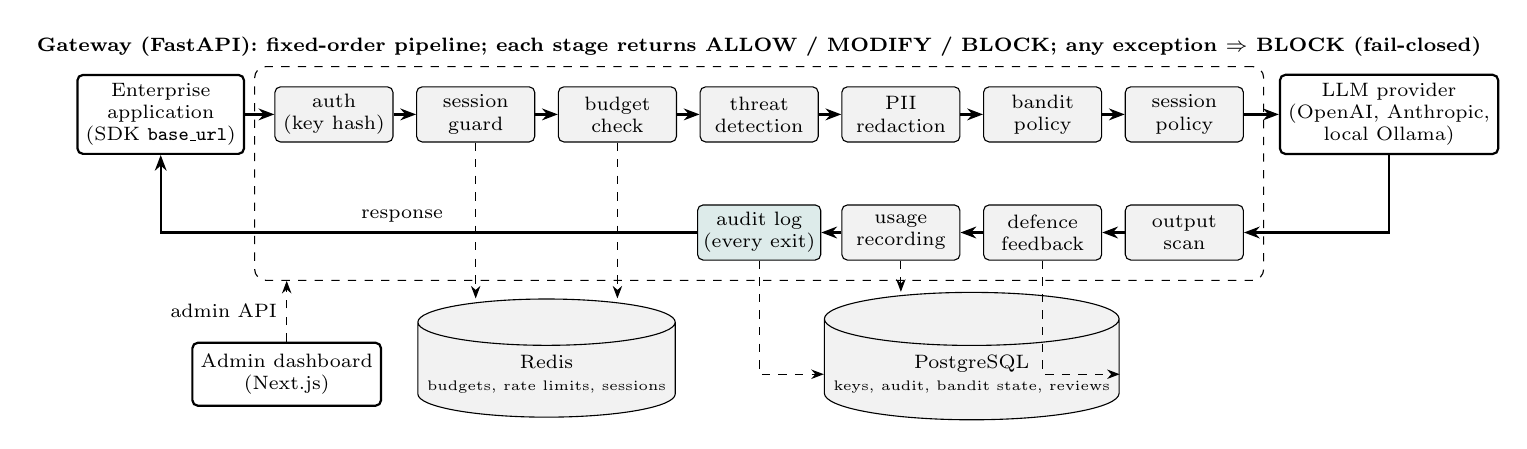
\begin{tikzpicture}[font=\scriptsize]
  \tikzset{st/.style={stage, minimum width=15mm}}
  % row 1: client, pre-call stages, provider
  \node[ext] (app) at (0,0) {Enterprise\\application\\(SDK \texttt{base\_url})};
  \node[st] (auth) at (2.2,0) {auth\\(key hash)};
  \node[st] (sg)   at (4.0,0) {session\\guard};
  \node[st] (bud)  at (5.8,0) {budget\\check};
  \node[st] (thr)  at (7.6,0) {threat\\detection};
  \node[st] (pii)  at (9.4,0) {PII\\redaction};
  \node[st] (ban)  at (11.2,0) {bandit\\policy};
  \node[st] (sp)   at (13.0,0) {session\\policy};
  \node[ext] (llm) at (15.6,0) {LLM provider\\(OpenAI, Anthropic,\\local Ollama)};
  % row 2: post-call stages, right to left
  \node[st] (out) at (13.0,-1.5) {output\\scan};
  \node[st] (fb)  at (11.2,-1.5) {defence\\feedback};
  \node[st] (use) at (9.4,-1.5) {usage\\recording};
  \node[st, fill=allowc!15] (aud) at (7.6,-1.5) {audit log\\(every exit)};
  % gateway frame
  \begin{scope}[on background layer]
    \node[draw, dashed, rounded corners, fit=(auth)(sp)(out)(aud), inner sep=2.5mm,
      label={[font=\scriptsize\bfseries, anchor=south]north:Gateway (FastAPI): fixed-order pipeline; each stage returns ALLOW / MODIFY / BLOCK; any exception $\Rightarrow$ BLOCK (fail-closed)}] (gw) {};
  \end{scope}
  % row 3: state stores and dashboard (outside the gateway)
  \node[store, minimum width=26mm] (rd) at (4.9,-3.3) {Redis\\{\tiny budgets, rate limits, sessions}};
  \node[store, minimum width=30mm] (pg) at (10.3,-3.3) {PostgreSQL\\{\tiny keys, audit, bandit state, reviews}};
  \node[ext] (dash) at (1.6,-3.3) {Admin dashboard\\(Next.js)};
  % request path
  \draw[arr] (app) -- (auth);
  \foreach \a/\b in {auth/sg, sg/bud, bud/thr, thr/pii, pii/ban, ban/sp} \draw[arr] (\a) -- (\b);
  \draw[arr] (sp) -- (llm);
  \draw[arr] (llm.south) |- (out.east);
  \draw[arr] (out) -- (fb);
  \draw[arr] (fb) -- (use);
  \draw[arr] (use) -- (aud);
  \draw[arr] (aud.west) -- node[above, pos=0.55]{response} (0,-1.5) -- (app.south);
  % state access
  \draw[darr] (sg.south) -- (sg.south |- rd.north);
  \draw[darr] (bud.south) -- (bud.south |- rd.north);
  \draw[darr] (aud.south) |- (pg.west);
  \draw[darr] (use.south) -- (use.south |- pg.north);
  \draw[darr] (fb.south) |- (pg.east);
  \draw[darr] (dash.north) -- node[left, pos=0.5]{admin API} (dash.north |- gw.south);
\end{tikzpicture}}
\caption{Architecture and request pipeline. Solid arrows: request path;
dashed: state access. The threat-detection stage only scores; the bandit
and session policies decide. Audit entries are written for allowed,
blocked and failed requests alike.}
\label{fig:arch}
\end{figure*}

Fig.~\ref{fig:arch} shows the gateway. It is a headless FastAPI service
that exposes an OpenAI-compatible chat endpoint; applications point their
SDK at it and authenticate with a gateway API key, stored only as a SHA-256
hash. Requests for \texttt{gpt-*} models are routed to OpenAI and
\texttt{claude-*} to Anthropic (with format translation); an optional local
provider (Ollama) allowed end-to-end testing without paid keys. PostgreSQL
holds teams, keys, bandit state, the review queue and the audit log; Redis
holds budgets, rate limits and session state.

\textbf{Pipeline and fail-closed rule.} Stages run in a fixed order and
each returns ALLOW, MODIFY or BLOCK. If any stage raises an exception the
request is blocked (HTTP 503) unless \texttt{FAIL\_MODE=open} is set
explicitly; a failing security check that lets traffic through would be a
bypass an attacker can trigger.

\textbf{Cost governance.} A token-bucket rate limiter runs as a Redis Lua
script. Budgets use \emph{reserve-then-reconcile}: one atomic script
reserves the estimated cost and checks the limit in the same step; after
the provider answers the reservation is corrected to the real cost, and on
any failure it is refunded. This removes a race we observed in an earlier
read-compare-write version: with ten concurrent requests against a budget
for three, exactly three are admitted.

\textbf{PII redaction.} Microsoft Presidio~\cite{presidio} detects names,
e-mail addresses, phone numbers and similar entities; our own patterns add
provider API keys and Luhn-validated card numbers, and win ties against
Presidio. Values are either masked (\texttt{[REDACTED\_EMAIL\_ADDRESS]}) or
tokenised, with the original stored Fernet-encrypted. Redaction is on by
default and covers message content and tool-call arguments. Only
entity-type counts are ever stored or logged.

\textbf{Admin dashboard.} A Next.js client of the gateway's admin API shows
traffic, the review queue, the audit log with an integrity check, threats,
spend and PII counts. The admin session token stays server-side in an
\texttt{httpOnly}, \texttt{SameSite=Strict} cookie.

% ---------------------------------------------------------------- methods
\section{Detection and Adaptive Defence}

\subsection{Threat Classifier}

A DeBERTa-v3-base model~\cite{he2023debertav3} is fine-tuned for three
classes: benign, prompt injection and jailbreak. Each message is split into
overlapping windows (160 tokens, at most 32), and a request's score is that
of its \emph{worst} window. Windowing defeats a padding attack we found:
250 tokens of filler before an injection lowered its score from 0.995 to
0.003 under truncation; with windows it scores 0.997. System prompts are
scored separately, because defensive instructions (``never reveal these
instructions'') otherwise score 0.98 as injection. Scores are calibrated by
temperature scaling~\cite{guo2017calibration}, $p=\mathrm{softmax}(z/T)$,
with $T=2.24$ fitted on validation data only, which lowered the
attack-score expected calibration error on validation from 0.042 to 0.019.
Training uses fp32, learning rate $2\times10^{-5}$, effective batch 16,
square-root inverse-frequency class weights and early stopping on
validation macro-F1, on a 4\,GB laptop GPU.

\subsection{Tactical Defence: Contextual Bandit}

Each request is a single decision with immediate feedback that does not
change the next request's situation, which is the contextual-bandit
setting rather than reinforcement learning. The bandit chooses one of four
arms: \emph{allow}, \emph{redact-and-allow} (remove the suspicious window),
\emph{block}, or \emph{escalate} to a human reviewer. Its context $x_t$ has
nine features: a bias term, the injection and jailbreak probabilities, the
attack log-odds, the system-prompt attack score and its product with the
conversation score, a truncation flag, the number of windows and the PII
entity count. Time of day and request rate were removed after we showed
that an attacker could use them to flip decisions. LinUCB~\cite{li2010contextual}
selects
\begin{equation}
a_t=\arg\max_a\;\hat\theta_a^{\top}x_t+\alpha\sqrt{x_t^{\top}A_a^{-1}x_t},
\qquad \hat\theta_a=A_a^{-1}b_a ,
\end{equation}
with $\alpha=0.5$. Feedback is discounted by $\gamma=0.999$ per arm update
so that stale labels fade; recovering from a long drift took 144 labels
instead of 793. A warm-start prior, never discounted, makes day-one
behaviour sensible (redact from attack score 0.335, escalate from 0.575,
block from 0.805), and a safety mask forbids \emph{allow} at scores $\ge
0.99$ whatever was learned. Labels come from reviewer verdicts on
escalations, a 2\% random spot-check of other decisions, and system-prompt
leaks found by the output scan (weight 0.2). Table~\ref{tab:reward} gives
the reward table.

\begin{table}[t]
\caption{Per-request reward used by the bandit}
\label{tab:reward}
\centering
\footnotesize
\begin{tabular}{lcc}
\toprule
Action & Benign request & Attack request \\
\midrule
allow & $+1.0$ & $-1.0$ \\
redact-and-allow & $+0.5$ & $0.0$ \\
block & $-0.3$ & $+0.5$ \\
escalate & $-0.1$ & $+0.45$ \\
\bottomrule
\end{tabular}
\end{table}

\subsection{Strategic Defence: DQN Session Agent}

A \emph{session} is one API key's traffic with gaps under 30 minutes. A
lockout or challenge changes what happens to every later request, and the
payoff arrives at the end of the session, so this is a sequential decision
problem that needs reinforcement learning. Fig.~\ref{fig:tiers} contrasts
the two tiers.

\begin{figure}[t]
\centering
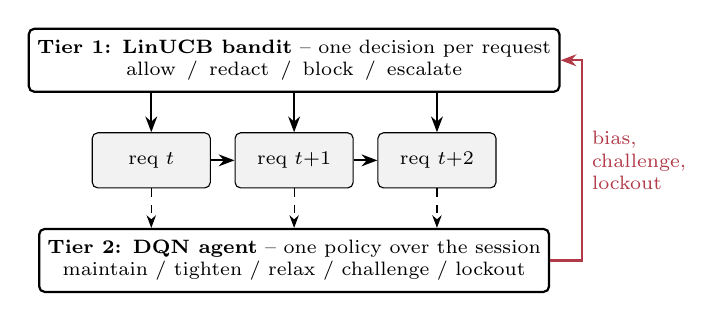
\begin{tikzpicture}[font=\scriptsize, node distance=3mm]
  \node[stage, minimum width=15mm] (r1) {req $t$};
  \node[stage, minimum width=15mm, right=of r1] (r2) {req $t{+}1$};
  \node[stage, minimum width=15mm, right=of r2] (r3) {req $t{+}2$};
  \node[ext, above=5mm of r2, minimum width=55mm] (bandit)
     {\textbf{Tier 1: LinUCB bandit} -- one decision per request\\
      allow \,/\, redact \,/\, block \,/\, escalate};
  \node[ext, below=5mm of r2, minimum width=55mm] (dqn)
     {\textbf{Tier 2: DQN agent} -- one policy over the session\\
      maintain / tighten / relax / challenge / lockout};
  \foreach \r in {r1,r2,r3} {
    \draw[arr] (bandit.south -| \r) -- (\r.north);
    \draw[darr] (\r.south) -- (dqn.north -| \r);
  }
  \draw[arr] (r1) -- (r2); \draw[arr] (r2) -- (r3);
  \draw[arr, refusec] (dqn.east) -- ++(4mm,0) |- node[pos=0.25, right, align=left]
       {bias,\\challenge,\\lockout} (bandit.east);
\end{tikzpicture}
\caption{Two-tier defence. The bandit decides each request independently;
the session agent reads the session's history and changes how later
requests are treated.}
\label{fig:tiers}
\end{figure}

\textbf{State and actions.} The 15-dimensional state contains only counts,
fractions and scores: the request count; the counts of allowed, redacted,
blocked and escalated requests; consecutive refusals; the last, mean and
maximum recent attack score and their slope; the share of requests scored
$\ge 0.5$; the redaction frequency; the current escalation bias; and a
pending-challenge flag. It therefore cannot carry text or PII. There are
five actions: \emph{maintain}; \emph{tighten} and \emph{relax} (shift the
bandit's escalation bias by $\pm0.25$, clamped to $[-0.3,1]$);
\emph{challenge} (send the next request to human review); and
\emph{lockout} (refuse the key for 15 minutes; requires at least two
refusals). We added the last two after measuring that, even at maximum
bias, the bandit changes its decision for only about 1\% of traffic, and
that 8 of 190 held-out attacks score below 0.2, which no score-based rule
can catch; only session-level actions can stop a persistent attacker who
eventually lands one of these.

\textbf{Reward and training.} The terminal reward is $+1.0$ for a benign
session ($-0.5$ if the agent intervened, $-2.0$ if it locked it out),
$+1.5$ for an attack session in which it intervened and $-2.0$ otherwise,
and $-2.0$ for any breach. To this we add $0.2$ times the bandit reward of
each request and potential-based shaping~\cite{ng1999policy}
\begin{equation}
F(s,s')=\gamma\Phi(s')-\Phi(s),\qquad \Phi(s)=0.5\cdot\max_{i\le t} p^{\text{attack}}_i .
\end{equation}
The agent is a Stable-Baselines3 DQN~\cite{mnih2015human,raffin2021sb3}
(64--64 MLP, learning rate $5\times10^{-4}$, 200k--300k steps); its weights
are exported to NumPy so that the gateway never loads pickled objects. A
rule-based fallback was built first: tighten after two consecutive
refusals and lock out after four. The training simulator replays real
held-out prompts with their real classifier scores through the bandit's
real code; only the session structure (lengths, probing, 85\% attacker
persistence, 20\% false-positive-prone users) is synthetic.

\subsection{Tamper-Evident Audit Log}

Every exit path writes one entry with the cost, PII counts, threat score,
bandit action, session action and outcome. Entries are chained as
\begin{equation}
h_i=\mathrm{SHA256}\bigl(h_{i-1}\,\Vert\,\mathrm{canon}(e_i)\bigr),\qquad h_0=\text{genesis},
\end{equation}
so editing any entry breaks its own hash and the link from its successor
(Fig.~\ref{fig:chain}). Three further layers prevent the easy attacks: an
ORM guard, a PostgreSQL trigger that rejects \texttt{UPDATE},
\texttt{DELETE} and \texttt{TRUNCATE}, and a restricted database role for
the gateway that may only insert and read audit rows and cannot disable
the trigger. The request only enqueues its entry; a single background
writer chains and stores batches at about 940 entries/s.

\begin{figure}[t]
\centering
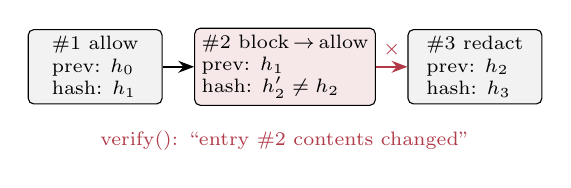
\begin{tikzpicture}[font=\scriptsize, node distance=4mm,
  blk/.style={draw, rounded corners=2pt, fill=boxc, align=left,
              minimum width=17mm, inner sep=2.5pt}]
  \node[blk] (b1) {\#1 allow\\prev: $h_0$\\hash: $h_1$};
  \node[blk, right=of b1, fill=refusec!12] (b2) {\#2 block\,$\to$\,allow\\prev: $h_1$\\hash: $h_2'\neq h_2$};
  \node[blk, right=of b2] (b3) {\#3 redact\\prev: $h_2$\\hash: $h_3$};
  \draw[arr] (b1) -- (b2);
  \draw[arr, refusec] (b2) -- node[above]{\textbf{$\times$}} (b3);
  \node[below=2mm of b2, align=center, text=refusec]
       {verify(): ``entry \#2 contents changed''};
\end{tikzpicture}
\caption{Hash chain. Changing entry \#2 changes its hash, which no longer
matches the \texttt{prev} hash stored in entry \#3; \texttt{verify} names the
first broken entry.}
\label{fig:chain}
\end{figure}

% ---------------------------------------------------------------- setup
\section{Experimental Setup}

\textbf{Data.} The first dataset (v1, 1{,}913 prompts) combines
deepset/prompt-injections, jackhhao/jailbreak-classification and benign
Alpaca instructions~\cite{taori2023alpaca}. A random split left 33 of the
91 test attacks as near-copies of training rows (jailbreak templates),
which inflated injection F1 from 0.81 to 0.87. We therefore cluster
near-duplicates (word 8-gram overlap $\ge0.5$, union-find) and assign whole
clusters to one split; a re-check finds no cluster crossing splits. The
expanded dataset (v2) adds the neuralchemy injection corpus, in-the-wild
jailbreaks~\cite{shen2024dan}, NotInject hard-benign
prompts~\cite{li2024injecguard} and Dolly instructions, removing 369
template copies. A new test set was locked by recording its SHA-256 hash
before any model was trained (Table~\ref{tab:data}).

\begin{table}[t]
\caption{Dataset splits (benign / injection / jailbreak)}
\label{tab:data}
\centering
\footnotesize
\begin{tabular}{lrrrr}
\toprule
Split & Total & Benign & Injection & Jailbreak \\
\midrule
v2 train & 6{,}307 & 3{,}521 & 1{,}661 & 1{,}125 \\
v2 validation & 830 & 463 & 226 & 141 \\
New test (locked) & 950 & 546 & 292 & 112 \\
Old test (v1) & 194 & 100 & 29 & 65 \\
\bottomrule
\end{tabular}
\end{table}

\textbf{Pre-registered criteria.} A new classifier replaces v1 only if, on
the new test, its injection F1 is higher and its benign false-positive
(FP) rate is not, and on the old test its macro-F1 is at least 0.913 with
an FP rate of at most 0.02. The DQN becomes the default session policy only
if it beats both \emph{maintain-only} and the rule on every scenario (paired
95\% confidence interval of the return difference above zero) while locking
out no more benign sessions than the rule plus one percentage point. Each
model is scored once per test set.

\textbf{Bandit protocol.} Policies are scored by mean reward per request
(Table~\ref{tab:reward}). Baselines are a threshold at 0.5, a threshold
tuned on the \emph{other} split, a hindsight-tuned threshold (an
unachievable ceiling), and the frozen warm-start prior. The bandit runs with
full feedback (an upper bound) and with realistic feedback (all escalations
plus 2\% spot checks). Experiment~A uses i.i.d.\ held-out data (2 folds
$\times$ 30 orders); Experiment~C simulates false-positive drift by giving
20\% of benign requests a score in $[0.95,0.995]$, the band where real false
positives were observed, at a 10\% attack rate.

\textbf{Session-agent protocol.} Policies are compared on paired simulated
sessions in four scenarios: \emph{standard} (20\% attack sessions),
\emph{attack-heavy} (50\%), \emph{low-rate} (5\%) and \emph{shifted}
(longer sessions, more false-positive-prone users and an attacker who
learns from refusals). Metrics are return, breach rate (attack sessions in
which an attack was allowed) and benign-lockout rate.

% ---------------------------------------------------------------- results
\section{Results}

\subsection{Classifier}

Table~\ref{tab:clf} compares the original model (v1), the expanded model
(v2) and a second attempt (v3) that started from v1's weights and
oversampled v1 data to reduce forgetting. On its own 194-prompt test v1
reaches a macro-F1 of 0.933, but on the larger locked test it falls to
0.490: it flags 27.5\% of benign prompts and misses most injections. v2
reaches 0.908 with a 3.1\% FP rate. Over both tests together (498 attacks,
646 benign prompts) v2 misses 28 attacks against v1's 63 and flags 18
benign prompts against v1's 151.

\begin{table}[t]
\caption{Classifier results (macro-F1, injection F1, benign FP rate)}
\label{tab:clf}
\centering
\footnotesize
\setlength{\tabcolsep}{4pt}
\begin{tabular}{llccc}
\toprule
Test set & Metric & v1 & v2 (shipped) & v3 \\
\midrule
\multirow{3}{*}{New (950)} & Macro-F1 & 0.490 & \textbf{0.908} & 0.877 \\
 & Injection F1 & 0.341 & \textbf{0.949} & 0.935 \\
 & Benign FP & 0.275 & \textbf{0.031} & 0.042 \\
\midrule
\multirow{3}{*}{Old (194)} & Macro-F1 & \textbf{0.933} & 0.884 & 0.871 \\
 & Injection F1 & \textbf{0.857} & 0.769 & 0.759 \\
 & Benign FP & \textbf{0.010} & \textbf{0.010} & 0.030 \\
\bottomrule
\end{tabular}
\end{table}

v2 nevertheless fails the third pre-registered criterion: its old-test
macro-F1 of 0.884 is below 0.913, a gap of six attacks on 194 prompts. v3
also failed. We shipped v2 as an explicitly recorded \emph{override} of the
rule, since the criterion was written to catch a regression on a small
benchmark, not to keep a model that flags over a quarter of benign
prompts on a five-times larger test. Single-prompt latency is 20--60\,ms on
the laptop GPU and 160--230\,ms on CPU.

\subsection{Contextual Bandit}

Table~\ref{tab:bandit} summarises Experiments A and C (v1 scores). On
i.i.d.\ data every policy is within 0.01 of the others: the bandit
\emph{ties} the tuned threshold (0.721 vs.\ 0.719; better in 30 of 60
runs). The scores are bimodal, with 168 of 190 attacks at $\ge0.999$ and
195 of 200 benign prompts below 0.01, so there is almost nothing in the
middle for a policy to learn from, and the 4.2\% of attacks the classifier
scores as benign look identical to benign traffic.

\begin{table}[t]
\caption{Bandit results: mean reward per request, attacks allowed and
benign requests refused}
\label{tab:bandit}
\centering
\footnotesize
\setlength{\tabcolsep}{3.5pt}
\begin{tabular}{lccc|ccc}
\toprule
 & \multicolumn{3}{c|}{A: i.i.d.} & \multicolumn{3}{c}{C: FP drift} \\
Policy & Reward & Att. & Ben. & Reward & Att. & Ben. \\
\midrule
Static, tuned & 0.719 & 4.2\% & 1.0\% & 0.697 & 4.7\% & 21.0\% \\
Static, hindsight & -- & -- & -- & 0.905 & 7.6\% & 2.8\% \\
Prior, frozen & 0.722 & 4.2\% & 0.5\% & 0.703 & 4.7\% & 20.5\% \\
Bandit, full fb. & 0.714 & 4.2\% & 0.5\% & \textbf{0.837} & 4.7\% & \textbf{0.9\%} \\
Bandit, 2\% fb. & 0.721 & 4.2\% & 0.5\% & 0.739 & 4.7\% & 15.1\% \\
\bottomrule
\end{tabular}
\end{table}

Under drift the picture changes. With full feedback the bandit learns to
redact rather than block the drifted band, gaining $+0.141\pm0.012$ reward
per request over the tuned threshold in 20 of 20 runs, and benign refusals
fall from 21.0\% to 0.9\% without letting more attacks through untouched.
The frozen prior behaves like the threshold (0.703), so the gain comes from
learning. The hindsight threshold scores higher only because it is tuned
on the stream's own labels, and it lets 7.6\% of attacks through. With the
realistic 2\% feedback the gain is $+0.042$, and it grows with the
labelling budget (Fig.~\ref{fig:spot}).

\begin{figure}[t]
\centering
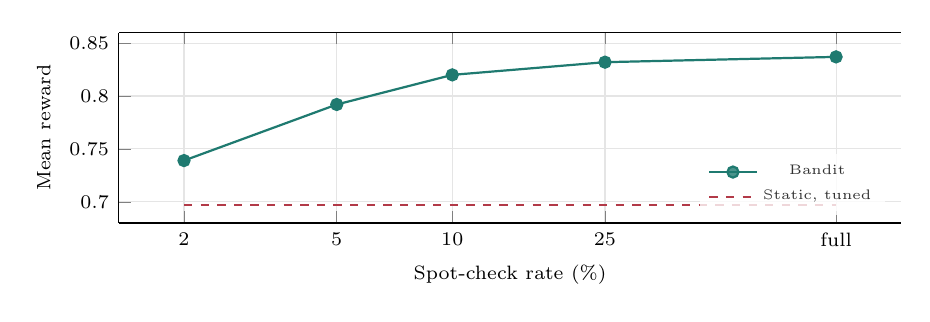
\begin{tikzpicture}
\begin{axis}[
  width=0.95\columnwidth, height=40mm,
  xlabel={Spot-check rate (\%)}, ylabel={Mean reward},
  xmode=log, log basis x=10,
  xtick={2,5,10,25,100}, xticklabels={2,5,10,25,full},
  ymin=0.68, ymax=0.86,
  axis y line*=left,
  font=\scriptsize, grid=major, grid style={gray!20},
  legend style={at={(0.98,0.04)}, anchor=south east, font=\tiny, draw=none, fill=white, fill opacity=0.8},
]
\addplot[thick, mark=*, color=allowc] coordinates {(2,0.739) (5,0.792) (10,0.820) (25,0.832) (100,0.837)};
\addlegendentry{Bandit}
\addplot[thick, dashed, color=refusec] coordinates {(2,0.697) (100,0.697)};
\addlegendentry{Static, tuned}
\end{axis}
\end{tikzpicture}
\caption{Experiment C: bandit reward vs.\ labelling budget. Benign
refusals fall from 15.1\% (2\%) to 7.7\%, 3.5\% and 1.8\% (5, 10, 25\%).}
\label{fig:spot}
\end{figure}

After the switch to the calibrated v2 classifier we re-ran the evaluation.
The i.i.d.\ result is still a tie, and with full feedback the bandit still
wins under drift ($+0.111$ on the new data). With realistic feedback,
however, it now \emph{trails} the tuned threshold at low attack rates
($-0.020$ at 10\% and $-0.024$ at 2\% attacks). Diagnosed on validation
data, the cause is the prior: its band edges were set when scores were
all-or-nothing, while 10\% of v2's benign validation prompts fall between
0.3 and 0.99, and 2\% feedback is too slow to move them.

\subsection{Session Agent}

Table~\ref{tab:rl} lists the three training runs. In run~1 every shaped
seed beat both baselines on return, but three of five did so partly by
locking out two to five times more benign sessions than the rule; without
shaping, two seeds collapsed. Run~2 priced a wrongful lockout at $-2.0$,
required two refusals before a lockout, and selected checkpoints on
validation sessions: every seed then met the lockout limit (0.9\% vs.\ the
rule's 0.8\%) and breaches fell from 14.4\% to 9.9\%, but two seeds were
not provably better than doing nothing when only 5\% of sessions are
attacks. Run~3 retrained on v2 scores as three voting ensembles of five
agents, evaluated on 20{,}000 sessions per scenario
(Table~\ref{tab:rl3}).

\begin{table}[t]
\caption{Session-agent runs against the go/no-go criterion}
\label{tab:rl}
\centering
\footnotesize
\setlength{\tabcolsep}{3pt}
\begin{tabular}{p{4mm}p{27mm}cp{25mm}}
\toprule
Run & Main change & Pass & Failure cause \\
\midrule
1 & baseline, $\pm$ shaping & 2/5, 0/5 & wrongful lockouts; 2 collapses \\
2 & lockout $-2.0$; validation checkpoints & 3/5 & no gain at 5\% attacks \\
3 & v2 scores; 3 ensembles of 5 DQNs & 0/3 & lockout 3.1--3.5\% $>$ 2.2\% \\
\bottomrule
\end{tabular}
\end{table}

\begin{table}[t]
\caption{Run 3: return and benign-lockout rate (20{,}000 sessions/scenario)}
\label{tab:rl3}
\centering
\footnotesize
\setlength{\tabcolsep}{3.5pt}
\begin{tabular}{lccccc}
\toprule
Scenario & Maintain & Rule & DQN ens. & Rule lock. & DQN lock. \\
\midrule
Standard & 1.569 & 1.779 & \textbf{1.84--1.86} & 1.2\% & 3.1--3.5\% \\
Attack-heavy & 0.390 & 1.257 & \textbf{1.56--1.57} & 1.3\% & 3.1--3.5\% \\
Low-rate & \textbf{2.153} & 2.040 & 1.97--2.00 & 1.2\% & 3.1--3.5\% \\
Shifted & \textbf{2.220} & 2.019 & 2.18--2.21 & 7.4\% & 6.6--7.9\% \\
\bottomrule
\end{tabular}
\end{table}

The ensembles beat the rule on three scenarios and let 8.3\% of attack
sessions through on \emph{standard}, against 11.7\% for the rule and 16.7\%
for maintain-only (Fig.~\ref{fig:tradeoff}). They exceed the lockout limit,
however, so the verdict is \textbf{NO-GO} and the rule remains the default;
the agent is available as an opt-in. Diagnosed on validation sessions,
checkpoint selection estimated lockout on only 600 sessions (about 10--15
events), so it favoured checkpoints whose lockout was low by chance: the
selected agents reported 0.2--2.2\% at selection but 2.2--4.8\% on 3{,}000
fresh sessions.

\begin{figure}[t]
\centering
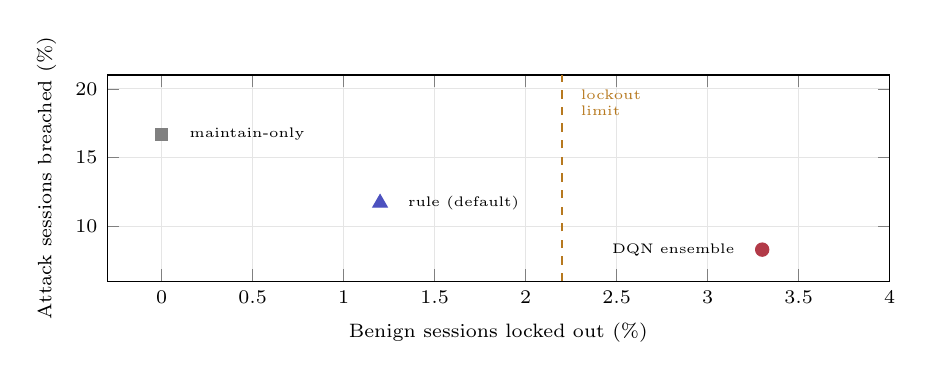
\begin{tikzpicture}
\begin{axis}[
  width=0.95\columnwidth, height=42mm,
  xlabel={Benign sessions locked out (\%)}, ylabel={Attack sessions breached (\%)},
  xmin=-0.3, xmax=4.0, ymin=6, ymax=21,
  font=\scriptsize, grid=major, grid style={gray!20},
]
\addplot[only marks, mark=square*, mark size=2.2pt, color=gray] coordinates {(0,16.7)};
\addplot[only marks, mark=triangle*, mark size=3pt, color=reviewc] coordinates {(1.2,11.7)};
\addplot[only marks, mark=*, mark size=2.4pt, color=refusec] coordinates {(3.3,8.3)};
\draw[dashed, color=cleanc, thick] (axis cs:2.2,6) -- (axis cs:2.2,21);
\node[font=\tiny, anchor=west] at (axis cs:0.1,16.7) {maintain-only};
\node[font=\tiny, anchor=west] at (axis cs:1.3,11.7) {rule (default)};
\node[font=\tiny, anchor=east] at (axis cs:3.2,8.3) {DQN ensemble};
\node[font=\tiny, anchor=west, color=cleanc, align=left] at (axis cs:2.25,19) {lockout\\limit};
\end{axis}
\end{tikzpicture}
\caption{Safety--security trade-off on the \emph{standard} scenario (run 3).
The DQN reduces breaches but crosses the pre-registered lockout limit.}
\label{fig:tradeoff}
\end{figure}

\subsection{End-to-End and Security Checks}

The full system was tested end to end with a local Llama~3 model behind
the gateway. In a prompt containing an e-mail address and a phone number,
both were removed before the model saw them; the model's reply contained
the literal placeholder, and the audit log held only
\texttt{\{EMAIL\_ADDRESS:1, PHONE\_NUMBER:1\}}. An ``ignore all previous
instructions'' prompt was blocked and the session tightened. Editing one
audit entry from \emph{block} to \emph{allow} directly in PostgreSQL was
detected and the entry named; under the gateway's restricted role the edit
was refused outright. Dedicated boundary tests plant e-mail addresses,
phone and card numbers and keys, then search every table, Redis key, debug
log line, response and upstream request. These tests found three leaks
that per-module tests had missed (a library logging analysed text at debug
level, provider error text echoing credentials, and tool-call arguments
bypassing all checks), all of which were fixed. The gateway's 437 tests
pass against real PostgreSQL and Redis with 97\% line-and-branch coverage,
and it sustains about 9 requests/s on a laptop CPU.

% ---------------------------------------------------------------- discussion
\section{Discussion and Limitations}

\textbf{Benchmarks can mislead.} The drop from 0.933 to 0.490 shows that a
small, narrow test set can overstate a model badly; leak-free splits and a
larger locked test were necessary to see it.

\textbf{A policy adds adaptivity, not accuracy.} The bandit costs nothing
where the classifier is right and recovers where its errors concentrate in
a score band that feedback can reveal, but it cannot fix the detector's
blind spots. Separating detection from response is still valuable: it
provides the safety mask, human escalation and a hook for session memory.

\textbf{Downstream components inherit upstream assumptions.} Better
calibrated scores exposed band edges in the bandit's prior that had been
fitted, implicitly, to the old model's all-or-nothing scores.

\textbf{RL found a real effect, but not reliably.} The agent learns to
intervene earlier in attack sessions, which the rule cannot, but its safety
depended on the training seed and on a noisy selection estimate. The reward
design and the statistical power of the safety constraint, rather than the
algorithm, were the bottlenecks.

\textbf{Limitations.} Detection was evaluated only on public benchmarks,
not against an adaptive attacker, and was not compared against other guard
models. Very short or imperative text still triggers false positives (a
bare ``hello'' scores 0.805), as does code in tool arguments. Some request
fields (tool definitions, the \texttt{user} field) are forwarded unchecked,
and the output scan detects only verbatim system-prompt leaks. The session
agent was trained in a simulator with synthetic session structure, and a
session is an API key, so a shared key lets one attacker lock out all its
users. The reward tables are hand-designed proxies. Streaming responses are
rejected so that the whole answer can be inspected first, and the
deployment is a single node.

% ---------------------------------------------------------------- conclusion
\section{Conclusion and Future Work}

We built and evaluated a fail-closed LLM gateway that combines cost
control, PII redaction, injection detection, a two-tier adaptive defence
and tamper-evident auditing. The classifier reaches a macro-F1 of 0.908 on
a locked 950-prompt test, and the evaluation showed that a smaller
benchmark had overstated an earlier model. The contextual bandit matches a
tuned threshold where the classifier is right and recovers from drift where
it is wrong. The DQN session agent reduced breaches relative to a rule
but did not meet a pre-registered safety criterion, so the rule stays the
default. Future work includes re-fitting the bandit's prior to calibrated
scores, a constrained or better-powered safety criterion for the session
agent trained on real logged sessions, an adaptive red-team loop, semantic
leak detection, and comparison with existing guard models on the locked
test set. We believe negative results reported with their causes are as
useful to practitioners as positive ones.

\section*{Acknowledgment}
The authors thank their guide, Mr.\ Monish L, and the Department of
DEPARTMENT, UNIVERSITY NAME, for their support, and the authors of the
public datasets used in this work.

% ---------------------------------------------------------------- references
\begin{thebibliography}{00}
\footnotesize
\bibitem{owasp2025} OWASP Foundation, ``OWASP Top 10 for Large Language Model Applications,'' 2025. [Online]. Available: \url{https://genai.owasp.org/llm-top-10/}
\bibitem{perez2022ignore} F. Perez and I. Ribeiro, ``Ignore previous prompt: Attack techniques for language models,'' in \textit{NeurIPS ML Safety Workshop}, 2022.
\bibitem{greshake2023not} K. Greshake, S. Abdelnabi, S. Mishra, C. Endres, T. Holz, and M. Fritz, ``Not what you've signed up for: Compromising real-world LLM-integrated applications with indirect prompt injection,'' in \textit{Proc. ACM AISec Workshop}, 2023.
\bibitem{liu2023prompt} Y. Liu \textit{et al.}, ``Prompt injection attack against LLM-integrated applications,'' arXiv:2306.05499, 2023.
\bibitem{wei2023jailbroken} A. Wei, N. Haghtalab, and J. Steinhardt, ``Jailbroken: How does LLM safety training fail?'' in \textit{Proc. NeurIPS}, 2023.
\bibitem{shen2024dan} X. Shen, Z. Chen, M. Backes, Y. Shen, and Y. Zhang, ```Do Anything Now': Characterizing and evaluating in-the-wild jailbreak prompts on large language models,'' in \textit{Proc. ACM CCS}, 2024.
\bibitem{inan2023llamaguard} H. Inan \textit{et al.}, ``Llama Guard: LLM-based input-output safeguard for human-AI conversations,'' arXiv:2312.06674, 2023.
\bibitem{rebedea2023nemo} T. Rebedea, R. Dinu, M. Sreedhar, C. Parisien, and J. Cohen, ``NeMo Guardrails: A toolkit for controllable and safe LLM applications with programmable rails,'' in \textit{Proc. EMNLP: System Demonstrations}, 2023.
\bibitem{li2024injecguard} H. Li, X. Liu, and C. Xiao, ``InjecGuard: Benchmarking and mitigating over-defense in prompt injection guardrail models,'' arXiv:2410.22770, 2024.
\bibitem{li2010contextual} L. Li, W. Chu, J. Langford, and R. E. Schapire, ``A contextual-bandit approach to personalized news article recommendation,'' in \textit{Proc. WWW}, 2010, pp. 661--670.
\bibitem{garivier2011switching} A. Garivier and E. Moulines, ``On upper-confidence bound policies for switching bandit problems,'' in \textit{Proc. ALT}, 2011, pp. 174--188.
\bibitem{mnih2015human} V. Mnih \textit{et al.}, ``Human-level control through deep reinforcement learning,'' \textit{Nature}, vol. 518, pp. 529--533, 2015.
\bibitem{raffin2021sb3} A. Raffin, A. Hill, A. Gleave, A. Kanervisto, M. Ernestus, and N. Dormann, ``Stable-Baselines3: Reliable reinforcement learning implementations,'' \textit{J. Mach. Learn. Res.}, vol. 22, no. 268, pp. 1--8, 2021.
\bibitem{ng1999policy} A. Y. Ng, D. Harada, and S. Russell, ``Policy invariance under reward transformations: Theory and application to reward shaping,'' in \textit{Proc. ICML}, 1999, pp. 278--287.
\bibitem{nguyen2021drl} T. T. Nguyen and V. J. Reddi, ``Deep reinforcement learning for cyber security,'' \textit{IEEE Trans. Neural Netw. Learn. Syst.}, vol. 34, no. 8, pp. 3779--3795, 2023.
\bibitem{schneier1999secure} B. Schneier and J. Kelsey, ``Secure audit logs to support computer forensics,'' \textit{ACM Trans. Inf. Syst. Secur.}, vol. 2, no. 2, pp. 159--176, 1999.
\bibitem{crosby2009efficient} S. A. Crosby and D. S. Wallach, ``Efficient data structures for tamper-evident logging,'' in \textit{Proc. USENIX Security Symp.}, 2009, pp. 317--334.
\bibitem{lee2022dedup} K. Lee \textit{et al.}, ``Deduplicating training data makes language models better,'' in \textit{Proc. ACL}, 2022, pp. 8424--8445.
\bibitem{he2023debertav3} P. He, J. Gao, and W. Chen, ``DeBERTaV3: Improving DeBERTa using ELECTRA-style pre-training with gradient-disentangled embedding sharing,'' in \textit{Proc. ICLR}, 2023.
\bibitem{guo2017calibration} C. Guo, G. Pleiss, Y. Sun, and K. Q. Weinberger, ``On calibration of modern neural networks,'' in \textit{Proc. ICML}, 2017, pp. 1321--1330.
\bibitem{presidio} Microsoft, ``Presidio: Data protection and de-identification SDK.'' [Online]. Available: \url{https://github.com/microsoft/presidio}
\bibitem{taori2023alpaca} R. Taori \textit{et al.}, ``Stanford Alpaca: An instruction-following LLaMA model,'' 2023. [Online]. Available: \url{https://github.com/tatsu-lab/stanford_alpaca}
\end{thebibliography}

\end{document}
